\section{Experiments}
\label{sec:experiments}

\subsection{Experimental setup}

We use two task families and several fixed predictors to vary how much
candidate-specific utility is visible to the selector. Traffic forecasting
provides the main controlled setting. Each target has a pool of candidate
sensors, a budget of four contexts, a history of twelve steps and a twelve-step
forecast horizon. Candidate pools mix highly correlated neighbours,
intermediate-correlation sensors and random distractors.

The first traffic predictor is a subset-capable ridge model fitted separately
for each target. The stronger traffic predictors are subset-capable neural
models trained with subset dropout so that arbitrary context sets are valid at
test time. They see the same candidate pools and evaluation episodes as the
ridge model, allowing predictor strength to change while the selection problem
stays fixed.

The second task family is demonstration selection for a frozen in-context image
classifier built on CLIP features. Candidate contexts are labelled
demonstrations, and utility is the reduction in query-batch cross-entropy. We
evaluate CIFAR-10, CIFAR-100, SVHN, EuroSAT and DTD with matched seeds and
candidate budgets.

Unless a scaling experiment changes them explicitly, all selectors use the same
candidate pool and budget within a comparison. Statistical tests are paired at
the target or benchmark level. Architecture details, data splits and the
complete per-run settings are given in the appendix.

\subsection{Theory validation}

Before comparing selectors, we test the statements that motivate their
parameterisation. For squared loss, the exact Bregman identity agrees with the
directly computed marginal to a maximum numerical discrepancy of
$3.3\times10^{-7}$. For softmax cross-entropy, the explicit sandwich of
\cref{prop:ce} has zero violations over $92{,}995$ candidate--state samples; the
largest observed Hessian eigenvalue reaches the theoretical constant $0.5$.
The first-order response term is strongly aligned with the true marginal
(Spearman $=.971$, $R^2=.853$), and adding response information to a held-out
utility model raises $R^2$ by $+.67$. The theory therefore predicts a signal
that can be measured directly before we study the full selector.

\begin{table}[t]
 \centering
 \small
 \caption{Numerical checks of the response--utility theory.}
 \label{tab:theory-validation}
 \begin{tabular}{lr}
  \toprule
  Check & Result\\
  \midrule
  Bregman identity, max. absolute error & $3.3\times10^{-7}$\\
  CE sandwich violations & $0/92{,}995$\\
  Max. CE Hessian eigenvalue & $.500$\\
  First-order term vs. marginal, Spearman & $.971$\\
  First-order term vs. marginal, $R^2$ & $.853$\\
  Held-out $R^2$ gain from response features & $+.67$\\
  \bottomrule
 \end{tabular}
\end{table}

\subsection{When utility is identifiable, response-aware selection wins}

We begin with the setting where candidate-level utility can be learned
reliably. The comparison fixes the candidate pools, predictor, episodes and
budget and evaluates content rules, fixed-set search, clustering, information
criteria, learned utility models and response-aware selection on the same
target--seed cells.

On METR-LA and PEMS-BAY, response-aware marginal routing achieves the highest
gain among all deployable methods in the detailed audit. Its gains are
$+.0146$ and $+.0557$, compared with $+.0080$ for pooling on METR-LA and
$+.0284$ for the cached-only router on PEMS-BAY. The response stage recovers value that remains inaccessible to content scores,
fixed subsets and response-free learned utilities.

\begin{table}[t]
 \centering
 \tablefont
 \caption{Selector audit in the identifiable traffic setting (32 targets,
 three seeds, 96 cells per dataset). Gains are relative to the anchor-only
 predictor with target-level 95\% intervals.}
 \label{tab:ridge-matrix}
 \begin{tabular}{lcccc}
  \toprule
  & \multicolumn{2}{c}{METR-LA} & \multicolumn{2}{c}{PEMS-BAY}\\
  \cmidrule(lr){2-3}\cmidrule(lr){4-5}
  Policy & Gain & 95\% CI & Gain & 95\% CI\\
  \midrule
  Sequential oracle & .1471 & $[.133,.161]$ & .1805 & $[.160,.201]$\\
  Standalone oracle & .1333 & $[.120,.146]$ & .1627 & $[.144,.181]$\\
  \textbf{Response-aware (ours)} & \textbf{.0146} & $[.009,.020]$ & \textbf{.0557} & $[.044,.067]$\\
  Pool all 16 & .0080 & $[.003,.013]$ & .0254 & $[.007,.044]$\\
  Cached-only router & .0042 & $[-.000,.009]$ & .0284 & $[.016,.041]$\\
  Standalone Utility & .0024 & $[-.002,.007]$ & .0272 & $[.013,.042]$\\
  Mutual information & $-.0055$ & $[-.010,-.001]$ & .0173 & $[.006,.029]$\\
  Random four & $-.0077$ & $[-.010,-.006]$ & .0095 & $[.003,.016]$\\
  k-means representatives & $-.0080$ & $[-.012,-.004]$ & .0043 & $[-.003,.011]$\\
  Facility location & $-.0163$ & $[-.023,-.009]$ & .0090 & $[-.005,.023]$\\
  Relevance (kNN) & $-.0165$ & $[-.024,-.009]$ & $-.0199$ & $[-.033,-.007]$\\
  DPP & $-.0166$ & $[-.022,-.011]$ & $-.0074$ & $[-.023,.008]$\\
  MMR & $-.0180$ & $[-.025,-.011]$ & $-.0249$ & $[-.044,-.006]$\\
  k-center & $-.0187$ & $[-.025,-.013]$ & .0043 & $[-.003,.011]$\\
  \bottomrule
 \end{tabular}
\end{table}

Several conventional selectors actively reduce prediction quality. Relevance
and MMR fall below the anchor-only predictor on both datasets; DPP, k-center,
k-means, facility location, random selection and mutual information are also
harmful on METR-LA. A DELIFT-style submodular representative rule remains below
pooling as well. The oracles still show large available value
($+.133$/$+.163$ standalone and $+.147$/$+.181$ sequential), so the selector
determines how much of that value reaches the predictor.

Candidate-pool growth provides a second positive mechanism check. As $K$ grows
from $4$ to $64$, absolute utility error improves while the true-marginal spread
shrinks faster: normalised error rises from $.403$ to $.739$ and the positive
top-two margin falls from $.220$ to $.024$. Adding compact predictor-response
features raises Spearman correlation with true utility from $.164$ to $.391$,
raises positive-utility AUC from $.649$ to $.834$, and reduces one-step regret
from $.0736$ to $.0569$. Thus response information helps precisely where a
content-only ordering becomes fragile.


\subsection{Why stronger predictors erase the ranking signal}

The theory predicts that routing becomes difficult when the fixed predictor
removes the systematic residual that distinguishes candidates. We test that
prediction directly.

\paragraph{Screening signal.}
With the nonlinear traffic predictor, the cached score has almost no
correlation with the true marginal at the first greedy steps
($+.005$, $-.049$, $-.019$). The shortlist recall is correspondingly close to
its random reference: $.26$--$.29$ at $q=4$ versus $.25$ for a random ranking,
and $.49$--$.53$ at $q=8$ versus $.50$. The response-aware stage is then asked
to choose from a shortlist that preserves little candidate-specific signal.

\paragraph{Within-state rankability.}
We next fit diagnostic models to the true marginals using all information
available before the target is known: anchor and candidate histories, candidate
identity, the response vector, response magnitude, and base--response
interactions. Across the evaluated cells, held-out $R^2$ averages $-.093$ and
the mean within-state rank correlation is $+.001$. In-sample and
label-permutation controls confirm that the pipeline can fit a signal when one
exists. The strong predictor leaves very little recoverable ordering
information in the observed state.

\paragraph{Pool geometry.}
Candidate novelty changes the picture. We construct three pools per dataset
whose leading candidates are drawn from the most correlated, middle, or least
correlated sensors. Relevance improves monotonically as the pool becomes less
redundant with the anchor (\cref{tab:pool-modes}).

\begin{table}[t]
 \centering
 \small
 \caption{Candidate novelty changes the value of relevance (8 targets, three
 seeds). Novelty is the share of candidate variance left unexplained by the
 anchor.}
 \label{tab:pool-modes}
 \begin{tabular}{lcccccc}
  \toprule
  & \multicolumn{3}{c}{METR-LA} & \multicolumn{3}{c}{PEMS-BAY}\\
  \cmidrule(lr){2-4}\cmidrule(lr){5-7}
  Pool head & novelty & relevance & pool all & novelty & relevance & pool all\\
  \midrule
  most correlated & .40 & $-.0086$ & $+.0116$ & .46 & $-.0333$ & $+.0112$\\
  moderate & .60 & $+.0006$ & $+.0070$ & .73 & $+.0117$ & $+.0064$\\
  least correlated & .79 & $+.0063$ & $+.0012$ & .95 & $+.0156$ & $+.0119$\\
  \bottomrule
 \end{tabular}
\end{table}

Across these controlled pool geometries, novelty correlates $+.80$ with
relevance gain. Every harmful cell has novelty at or below $.46$ and every
helpful cell has novelty at or above $.60$. The absolute threshold is
deployment-specific, but the direction is stable: relevance becomes useful as
the pool contributes more information beyond the anchor.

\paragraph{Predictor strength as a mechanism.}
We build a ladder of predictors on matched METR-LA cells. Anchor error decreases
as the neural predictors become stronger, while the fraction of oracle value
realized by routing falls sharply (\cref{tab:ladder}).

\begin{table}[t]
 \centering
 \small
 \caption{Predictor-strength ladder on METR-LA (eight targets, one seed). Lower
 anchor MSE indicates a stronger predictor.}
 \label{tab:ladder}
 \begin{tabular}{lccccc}
  \toprule
  Expert & Anchor MSE & Standalone oracle & Sequential oracle & Learned gain & Realized share\\
  \midrule
  ridge & .3782 & $+.1535$ & $+.1687$ & $+.0313$ & $.198$\\
  transformer, 1 layer & .3721 & $+.0835$ & $+.0961$ & $+.0222$ & $.268$\\
  masked-mean MLP & .3625 & $+.1002$ & $+.1198$ & $+.0273$ & $.243$\\
  transformer, 2 layers & .3578 & $+.0923$ & $+.1044$ & $+.0168$ & $.177$\\
  transformer, 3 layers & .3562 & $+.0902$ & $+.1060$ & $+.0075$ & $.063$\\
  \bottomrule
 \end{tabular}
\end{table}

Within the neural family, the oracle opportunity stays in a narrow range while
the realized share drops from roughly a quarter to a few percent as the anchor
improves. Structural headroom alone does not predict this change. Across the
six traffic benchmarks, targets with similar oracle headroom can have very
different gains over pooling. The selector succeeds when the predictor leaves a
systematic residual that the response can reveal.


\subsection{Stronger predictors preserve opportunity while realizable gain shrinks}

The full strong-predictor comparison makes the same point at the policy level
(\cref{tab:strong-backbone}). Sequential-oracle gains remain large on both
datasets, yet the deployable selectors cluster near pooling. On PEMS-BAY,
pooling is significantly above every learned alternative. On METR-LA, the
response-aware family remains statistically tied with pooling and stays closer
to it than the response-free learned rules.

\begin{table}[t]
 \centering
 \small
 \caption{Strong-predictor comparison on 16 targets and three seeds. Gains are
 loss reductions relative to the anchor-only predictor.}
 \label{tab:strong-backbone}
 \begin{tabular}{lcc}
  \toprule
  Policy & METR-LA & PEMS-BAY\\
  \midrule
  Anchor only & .0000 & .0000\\
  Random four & .0062 & .0163\\
  Relevance & .0070 & .0108\\
  MMR & .0077 & .0113\\
  Diversity (DPP) & .0091 & .0142\\
  Standalone Utility & .0069 & .0139\\
  Cached-only router & .0076 & .0135\\
  Response-aware, frozen head & .0097 & .0130\\
  Response-aware, theory-shaped head & .0107 & .0125\\
  Pool all 16 & \textbf{.0133} & \textbf{.0225}\\
  Mutual information & .0134 & ---\\
  Policy-gradient selector & $-.0041$ & ---\\
  Standalone oracle & .0904 & .0880\\
  Sequential oracle & .1051 & .1037\\
  \bottomrule
 \end{tabular}
\end{table}

The budget sweep shows that this gap is not caused by choosing too few or too
many contexts. With true marginals, the best budget is three and the oracle
gain decreases after that point. Random subsets improve as more contexts are
added. The two curves move in opposite directions, exposing a large gap between
what perfect information could achieve and what a selector can recover from the
available observations.

Candidate-library scaling sharpens the result. Holding the budget fixed while
growing the library from 16 to 128 candidates increases the oracle gain from
$+.0851$ to $+.1196$, yet the learned router falls from $+.0076$ to $-.0025$
(\cref{tab:pool-size}). More candidates create more oracle opportunity and a
harder ranking problem at the same time.

\begin{table}[t]
 \centering
 \small
 \caption{Candidate-library scaling with the strong predictor (METR-LA,
 16 matched cells, budget four).}
 \label{tab:pool-size}
 \begin{tabular}{lcccc}
  \toprule
  Candidates & Pool all & Router & Random four & Oracle\\
  \midrule
  $16$  & $+.0057$ & $+.0076$ & $+.0005$ & $+.0851$\\
  $32$  & $+.0128$ & $+.0031$ & $+.0049$ & $+.0987$\\
  $64$  & $+.0081$ & $-.0033$ & $+.0018$ & $+.1180$\\
  $128$ & $+.0042$ & $-.0025$ & $-.0006$ & $+.1196$\\
  \bottomrule
 \end{tabular}
\end{table}

\begin{figure*}[t]
  \centering
  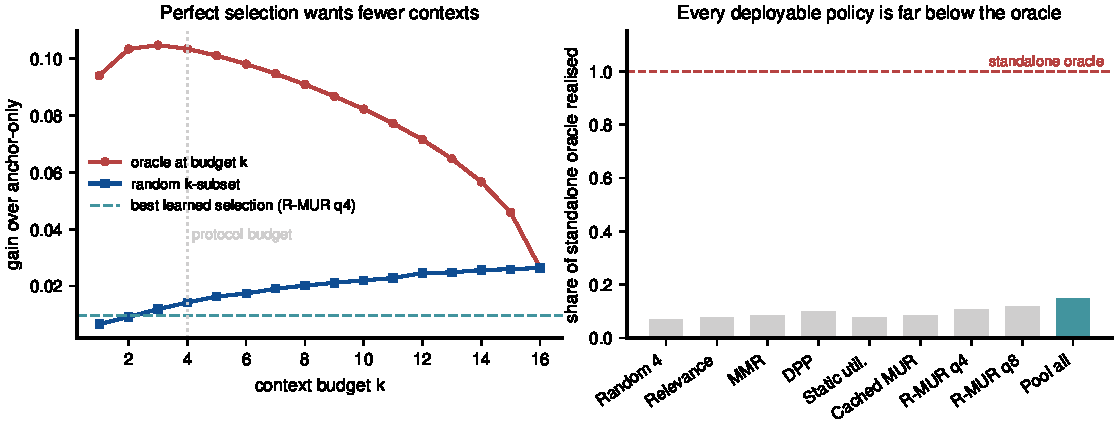
\includegraphics[width=0.98\textwidth]{figures/fig7_budget_gap.pdf}
  \caption{Oracle opportunity and realizable value separate under the strong
  predictor. The oracle prefers a small budget, while random subsets improve as
  more contexts are included.}
  \label{fig:budget-gap}
\end{figure*}

Removing the shortlist does not recover the missing value. Setting $q=K$ changes
the response-aware result by only $+.0012$ with an interval that includes zero.
The same conclusion survives backward elimination, harmful-pool construction,
response-geometry heuristics and an episode-level confidence analysis. Those
stress tests are reported in the appendix. Together they place the bottleneck
in the information available for ranking, not in the search direction or the
two-stage implementation.


\subsection{Pool geometry yields an adaptive fallback}

The third measurement converts into the policy of \cref{eq:adaptive-rule}. With
the threshold chosen on half of the targets and then held fixed, the rule
reaches $+.0081\;[+.0017,+.0138]$ on METR-LA and $+.0129\;[-.0066,+.0329]$ on
PEMS-BAY, against $-.0006$ and $-.0020$ for fixed relevance and $+.0066$ and
$+.0098$ for always pooling everything; it captures $87\%$ and $67\%$ of an
oracle that picks the better of the two policies per cell. The selected threshold is stable across splits on METR-LA ($[.45,.55]$ in
$198$ of $200$) and less stable on PEMS-BAY, where it often reaches the lower
end of the search grid. The threshold is therefore fitted within each
deployment. The rule clearly improves on fixed relevance on METR-LA and shows
the same direction on PEMS-BAY. Its purpose is practical: it replaces a harmful
default with a geometry-aware choice, while learned marginal-utility routing
remains the stronger option when labelled training states are available.

\subsection{Demonstration selection separates ranking from stopping}

In demonstration selection the predictor consumes labelled examples, so the
mechanism of \cref{sec:theory} applies with a different information type. The
predictor is genuinely in-context: mean accuracy rises from $.966$ to $.983$ on
CIFAR-10, $.812$ to $.997$ on CIFAR-100, $.693$ to $.996$ on SVHN, $.946$ to
$.986$ on EuroSAT and $.728$ to $.921$ on DTD when four relevant demonstrations
are added, and the farthest demonstrations are worse than random ones.

\begin{table}[t]
 \centering
 \small
 \caption{Demonstration-selection results. Values are mean cross-entropy
 reductions (nats) at shortlist size four; $\Delta$ columns compare with the
 response-free learned routers.}
 \label{tab:second-family}
 \begin{tabular}{lccccc}
  \toprule
  Benchmark & Ours & Static & Cached & $\Delta$Static & $H_{\mathrm{state}}$\\
  \midrule
  CIFAR-10 & .0643 & .0482 & .0433 & $+.0160$ & .000\\
  CIFAR-100 & .5247 & .5769 & .5381 & $-0.0522$ & .000\\
  SVHN & .8809 & .7530 & .7688 & $+.1279$ & .000\\
  EuroSAT & .1294 & .1074 & .1125 & $+.0221$ & .000\\
  DTD & .3322 & .5981 & .6478 & $-0.2658$ & .000\\
  \bottomrule \end{tabular}
\end{table}

The frozen head passes the per-benchmark criterion on three of five benchmarks
and fails on CIFAR-100 and DTD, where a nearest-neighbour relevance rule is
already within a fraction of a percent of the oracle. The family also exposes
a boundary condition: the sequential and standalone oracles coincide to four
decimals ($H_{\mathrm{state}}\le 5\times10^{-4}$), because the candidate pools
contain no redundant demonstrations, so selecting the best standalone
demonstrations is already optimal.

\paragraph{Scoring-head ablation.} We iterated on the scoring head to test
whether the failure is one of functional form. A redundancy-structured variant
of the pools was built first (four clusters of three near-duplicate
demonstrations); measured redundancy was real --- a second member of a cluster
retains only $6.7$--$42\%$ of the first member's marginal --- yet the
sequential oracle still does not meaningfully exceed the standalone oracle,
because utility in this family is label-driven: replacing candidate
\emph{features} by noise costs only about $18\%$ of the first-member marginal,
while equalising \emph{labels} flips every marginal negative. For that
predictor the utility is nearly a function of the label multiset of the
selected set, so no pool geometry can make it state-conditioned.

Replacing the predictor with a query-comparative one (a learned-metric
prototype in which a demonstration can only help through its image content)
closes that shortcut: the second-member marginal falls to $0.12$--$0.78\%$ of
the first, and pooled state-conditioned headroom becomes genuinely positive
($+.0126\;[+.0019,+.0239]$). In that setting the theory-shaped bilinear head of
\cref{eq:bilinear-head} ranks the true marginal better than the scalar head on
four of five benchmarks (mean within-state Spearman $.375$ against $.156$;
top-one agreement $.67$ against $.08$ on CIFAR-100) and gives the largest pooled
forced-budget contrast against Standalone Utility of the three heads
($+.0605\;[-.0036,+.1343]$, three of five per-benchmark intervals above zero).
The association between response magnitude and marginal utility changes sign
across benchmarks ($+.257$ on CIFAR-10 and $-.590$ on CIFAR-100), while the
fixed curvature term assumes one sign. Allowing a learned signed coefficient
moves that coefficient from its $-.25$ initialization to positive values on
four of five benchmarks, confirming the sign change. Performance remains in the
same narrow band. Across scalar, curvature-corrected, bilinear and signed
bilinear heads, the main variation comes from the observable signal available
to the scorer, while extra parameterization changes the ordering only modestly.

\subsection{Efficiency and deployment}

A full $B$-step episode can spend up to $B(1+q)$ predictor evaluations under
the uncached accounting used by this benchmark: the measured totals are $20$
rows per episode at $q=4$ and $36$ at $q=8$, against about $64$ for reranking
the full pool and $17$ for the standalone-oracle reference. Measured at deployment batch size on the same cell,
the response-aware stage costs $.74$, $1.19$, $1.59$ and $2.65$ milliseconds
per episode for $q=2,4,8,16$, against $1.70$ milliseconds for the sequential
oracle and $.03$ milliseconds for cached screening alone
($0$ expert evaluations), and it raises peak device memory from $90$ to
$173$ megabytes. The shortlist keeps the response stage compact: $q=4$ uses roughly one third
of the full-pool predictor evaluations while staying close to the best observed
routing result in the strong-predictor setting.

\paragraph{Deployment pilot.}
The method can be evaluated before a full rollout with a small labelled pilot.
Across the six traffic deployments, a pilot of 24 targets reproduces the
full-sample routing verdict 96\% of the time. Splitting the pilot in half gives
a high-confidence self-check: when both halves resolve in the same direction,
agreement with the full deployment reaches 99\% or higher at the evaluated
pilot sizes. Under a later time split, the target-level effect remains
directionally stable (within-dataset correlation $+.596$ and 81\% sign
agreement), while the dataset-level significance call agrees on four of six
datasets. The pilot is most useful for clear cases; marginal cases benefit from more
labelled targets.
